\documentclass[11pt]{article}

\usepackage[margin=1in]{geometry}
\usepackage[utf8]{inputenc}
\usepackage[T1]{fontenc}
\usepackage{graphicx}
\usepackage{booktabs}
\usepackage{hyperref}
\usepackage{amsmath}
\usepackage{float}
\usepackage{enumitem}
\usepackage{setspace}

\onehalfspacing

\title{StreamCab: Real-Time Taxi Fare Intelligence with Kafka, Spark, and XGBoost}
\author{
Your Name \\
Group Member 1 \\
Group Member 2 \\
Group Member 3
}
\date{\today}

\begin{document}
\maketitle

\begin{abstract}
This paper presents StreamCab, an end-to-end data engineering and machine learning system for real-time taxi analytics and short-term fare prediction. The pipeline replays historical New York City taxi trips into Apache Kafka, processes and aggregates the stream using Apache Spark Structured Streaming, stores results in PostgreSQL, and serves predictions through a dashboard interface. We describe the architecture, data processing methodology, model training strategy, and performance outcomes, then discuss practical lessons learned about reliability, memory constraints, and deployment trade-offs in single-node environments.
\end{abstract}

\section{Introduction}
Urban transportation data is high-volume, time-sensitive, and geographically heterogeneous. Static batch reports are often insufficient for operational decisions such as where demand is increasing and what pricing behavior to expect in the next few minutes. This project investigates whether a compact local stack can deliver near real-time analytics and prediction from historical taxi records replayed as live events.

The objectives of StreamCab are:
\begin{itemize}[leftmargin=1.5em]
    \item Build a reproducible streaming pipeline from data ingestion to visualization.
    \item Produce interpretable zone-level aggregate metrics over short windows.
    \item Train and serve a practical fare predictor under memory constraints.
    \item Evaluate model quality against a baseline and report engineering trade-offs.
\end{itemize}

\section{Related Work / Background}
Streaming architectures commonly use Kafka for event transport, Spark Structured Streaming for stateful transformations, and SQL databases for serving curated outputs \cite{kafka,spark}. Gradient-boosted trees, especially XGBoost, are widely used for tabular prediction due to strong accuracy-speed trade-offs \cite{xgboost}.

Compared to distributed cloud deployments, this project emphasizes local reproducibility and careful memory-aware design. The training pipeline uses batched parquet processing and continued model updates to support large datasets on limited RAM.

\section{System Architecture and Design}
\subsection{Architecture Overview}
The system has six services: PostgreSQL, Kafka (+ producer), Spark/predictor/dashboard app container, consumer, one-shot trainer, and Kafka Control Center.

\begin{figure}[H]
    \centering
    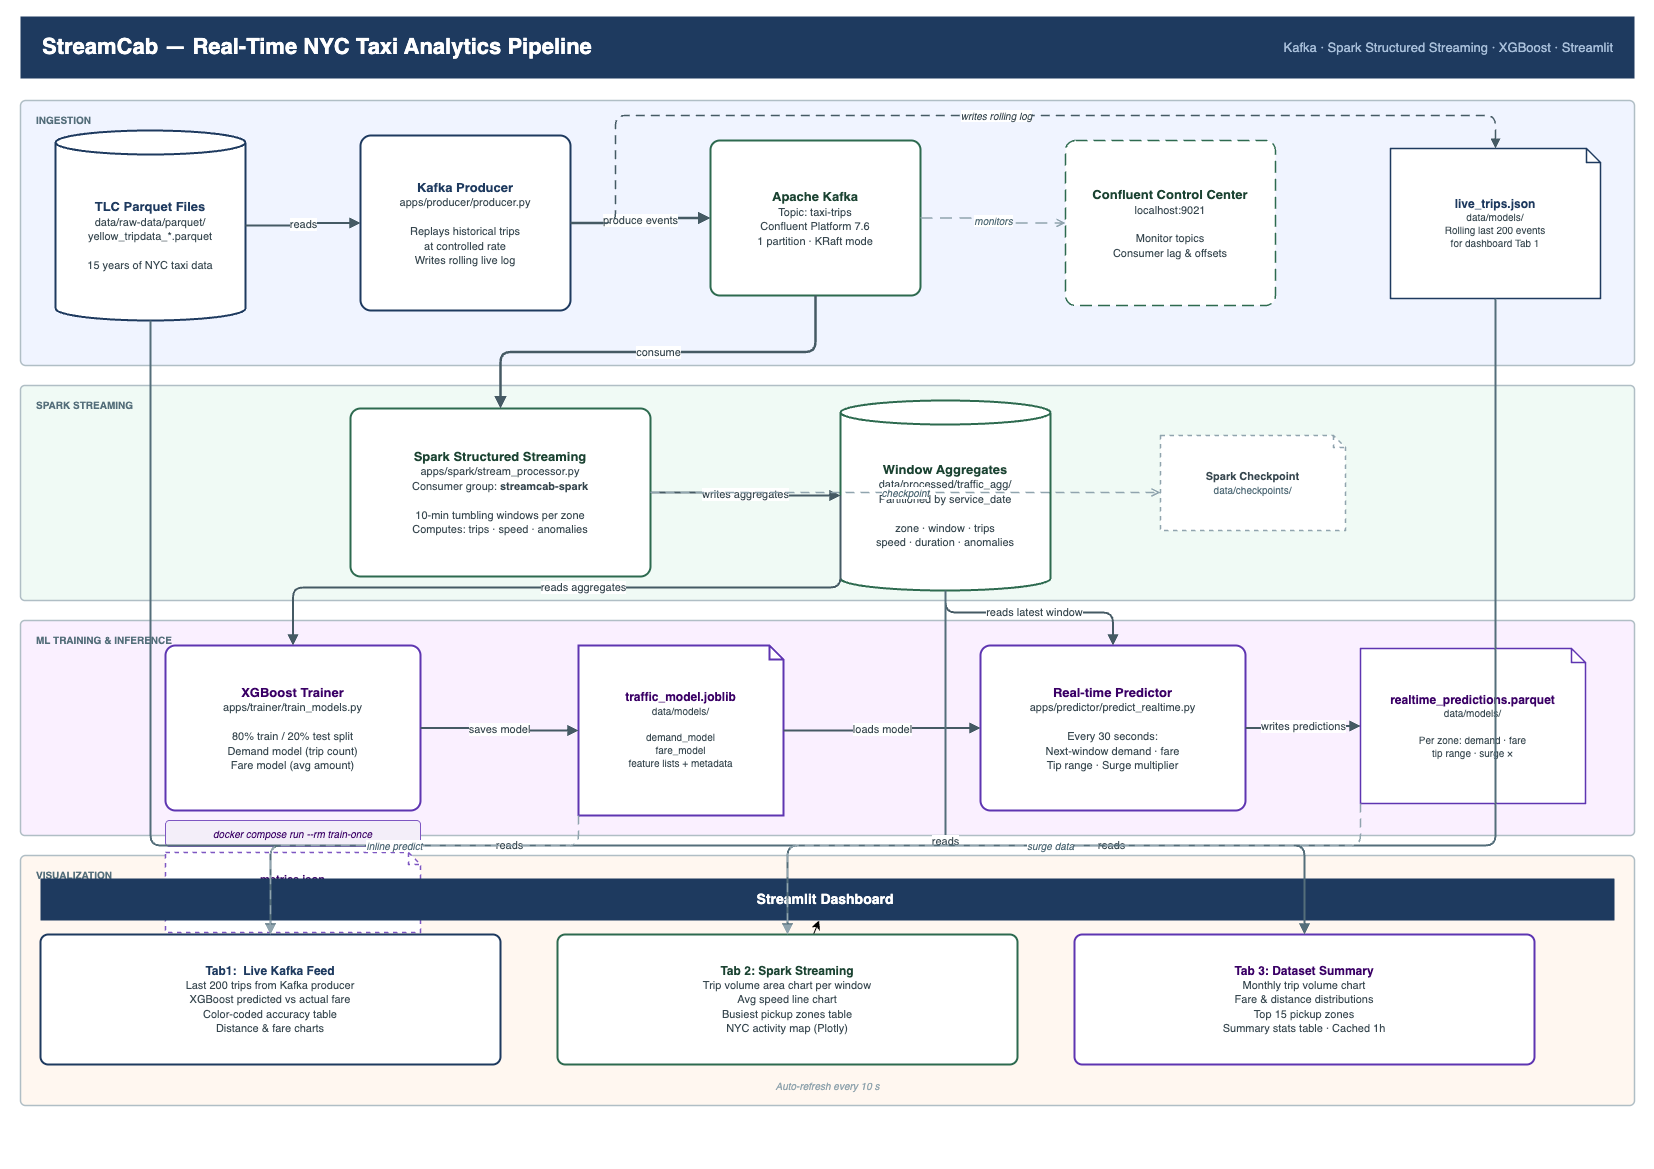
\includegraphics[width=0.95\linewidth]{../assets/architecture.png}
    \caption{StreamCab end-to-end architecture.}
    \label{fig:architecture}
\end{figure}

\subsection{Component Responsibilities}
\begin{itemize}[leftmargin=1.5em]
    \item \textbf{Producer:} Streams normalized trip events from parquet in replay loops.
    \item \textbf{Kafka:} Buffers and distributes trip events to downstream consumers.
    \item \textbf{Spark Structured Streaming:} Applies cleaning rules and windowed zone aggregations.
    \item \textbf{PostgreSQL:} Stores live trips, traffic aggregates, and prediction outputs.
    \item \textbf{Trainer:} Builds XGBoost fare model from historical aggregates.
    \item \textbf{Predictor + Dashboard:} Performs periodic inference and displays live analytics.
\end{itemize}

\subsection{Tools Not Covered in Class (Brief Intro)}
If needed for course context:
\begin{itemize}[leftmargin=1.5em]
    \item \textbf{Apache Kafka:} Distributed event log for pub/sub data streaming.
    \item \textbf{Spark Structured Streaming:} Incremental DataFrame processing with watermarks and windows.
    \item \textbf{JDBC/Psycopg integration:} Database connectivity between Spark/Python services and PostgreSQL.
\end{itemize}

\section{Data Collection and Processing}
\subsection{Data Source}
Primary data comes from publicly available NYC TLC yellow taxi trip records (monthly parquet files).

\textbf{Data source link:} \url{https://www.nyc.gov/site/tlc/about/tlc-trip-record-data.page} \cite{tlc}

\subsection{Collection Procedure}
\begin{enumerate}[leftmargin=1.5em]
    \item Download selected monthly parquet files.
    \item Store files under project raw-data directory.
    \item Replay rows as pseudo-live events through Kafka.
\end{enumerate}

\subsection{Schema and Metadata}
\textbf{Raw/event schema (core fields):}
\begin{itemize}[leftmargin=1.5em]
    \item pickup\_datetime, dropoff\_datetime
    \item passenger\_count, trip\_distance
    \item pu\_location\_id, do\_location\_id
    \item total\_amount, emitted\_at
\end{itemize}

\textbf{Windowed aggregate schema:}
\begin{itemize}[leftmargin=1.5em]
    \item window\_start/window\_end, pu\_location\_id, trip\_count
    \item avg\_speed\_mph, avg\_duration\_min, avg\_trip\_distance
    \item avg\_total\_amount, anomaly\_count
\end{itemize}

\subsection{Processing Method (Inputs and Outputs)}
Inputs are raw parquet trip files and zone centroid metadata. Processing includes type normalization, quality filters, temporal feature extraction, and sliding-window aggregation. Outputs include:
\begin{itemize}[leftmargin=1.5em]
    \item Streaming aggregate table for current operational state.
    \item Trained fare model artifact and evaluation metrics.
    \item Prediction records consumed by dashboard visualizations.
\end{itemize}

\section{Model Training and Inference Strategy}
\subsection{Baseline and Features}
The baseline predicts mean fare by pickup zone and hour. The XGBoost model uses zone ID, hour/day/weekend flags, average distance, duration, speed, and trip count.

\subsection{Memory-Aware Training}
To support large datasets on limited memory, the trainer:
\begin{itemize}[leftmargin=1.5em]
    \item reads parquet in bounded batches,
    \item computes additive aggregate statistics,
    \item finalizes means after grouped reductions,
    \item applies continued training across chronological batches,
    \item selects the best validation checkpoint for final artifact.
\end{itemize}

\section{Results and Analysis}
\subsection{Quantitative Results}
Replace or update with your final run metrics.

\begin{table}[H]
\centering
\begin{tabular}{lcc}
\toprule
Model & MAE & MAPE (\%) \\
\midrule
Baseline (zone-hour mean) & 1.9891 & 15.43 \\
XGBoost (test) & 0.4851 & 3.42 \\
\bottomrule
\end{tabular}
\caption{Example model performance summary.}
\label{tab:metrics}
\end{table}

\subsection{Dashboard and Analytics Outputs}
Include screenshots or figures for:
\begin{itemize}[leftmargin=1.5em]
    \item Live trips per minute
    \item Zone ranking and surge signals
    \item City map activity visualization
\end{itemize}

\begin{figure}[H]
    \centering
    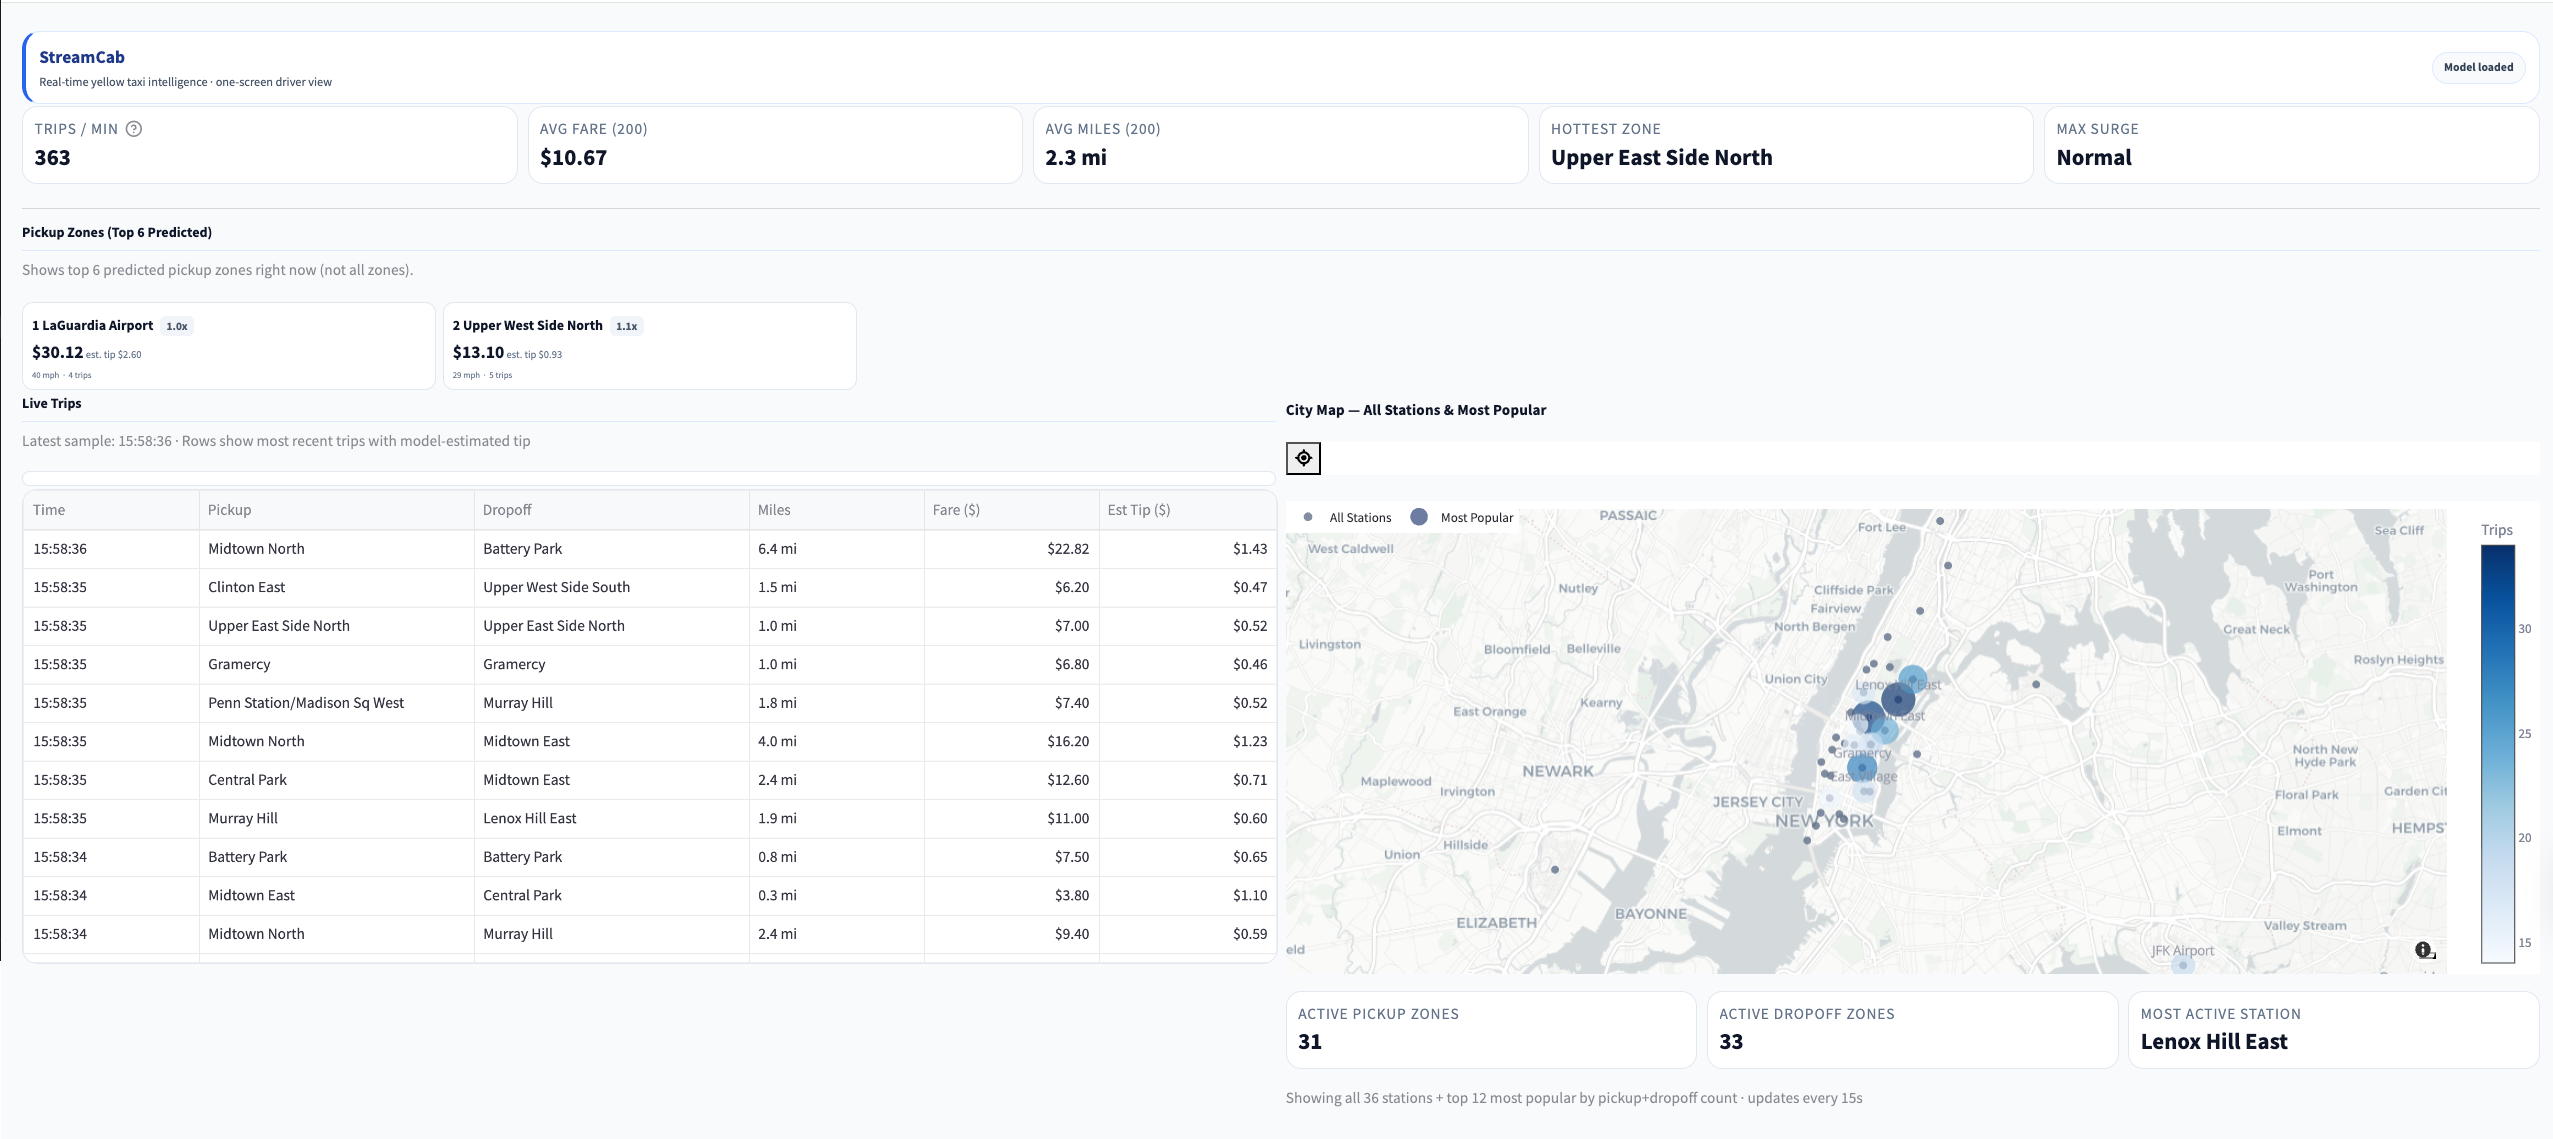
\includegraphics[width=0.95\linewidth]{../assets/app.png}
    \caption{StreamCab dashboard showing live trip table, zone-level insights, and map-based analytics.}
    \label{fig:dashboard}
\end{figure}

\subsection{Discussion}
The pipeline demonstrates that practical near real-time analytics can be achieved in a local setup when ingestion, processing, and training are designed for bounded memory and idempotent writes. SQL-side narrowing for predictor reads and stream checkpointing significantly improve operational stability.

\subsection{Limitations and Threats to Validity}
Although the quantitative results are strong, several limitations affect generalization and operational confidence. First, the stream is a replay of historical data rather than a true live feed, so observed latency and throughput may differ from production systems with bursty arrival patterns, schema drift, and upstream outages. Second, zone-level aggregates improve model stability but can hide fine-grained effects such as street-level congestion, event-driven anomalies, and rare pickup/dropoff combinations.

The evaluation window is also constrained by selected months and filtering rules. If market conditions shift (fuel prices, policy changes, seasonality, or weather shocks), model error can increase without immediate visibility. Future iterations should include explicit drift indicators (feature distribution shift, residual monitoring, and alarm thresholds) to ensure model performance remains within acceptable bounds. Finally, local single-node deployment simplifies reproducibility, but it does not fully represent fault domains and scaling behavior in distributed environments.

\subsection{Reproducibility and Operational Notes}
To support reproducibility, all services are containerized and orchestrated through Docker Compose with deterministic startup dependencies. The project separates concerns across producer, streaming processor, consumer, trainer, and dashboard services. This isolation reduces coupling and makes it easier to troubleshoot failures by layer. The end-to-end runbook consists of: (1) downloading raw TLC parquet data, (2) launching services, (3) running one-shot training, (4) starting replay/streaming, and (5) validating outputs in PostgreSQL and the dashboard.

Operationally, two implementation choices were especially important. The first is checkpointed stream processing with bounded windows, which limits duplicate writes and supports restart safety. The second is memory-aware training via batched parquet reads and incremental model updates, which enables full-dataset learning on commodity hardware. For teams extending this project, we recommend adding lightweight data quality contracts at ingest time (null/negative checks, timestamp sanity, and schema assertions) and documenting expected service-level objectives for latency and prediction freshness.

The architecture can be extended incrementally: move stateful processing to a managed cluster, introduce model registry/versioning, and add automated backtesting before promoting new models. These steps preserve the current educational value while improving production readiness.

\section{Conclusion and Key Takeaways}
\textbf{What worked well:}
\begin{itemize}[leftmargin=1.5em]
    \item Modular services and reproducible local orchestration.
    \item Streaming aggregates as robust prediction features.
    \item Strong tabular prediction performance with XGBoost.
\end{itemize}

\textbf{Main challenges:}
\begin{itemize}[leftmargin=1.5em]
    \item Large data volume vs local memory constraints.
    \item Reliability semantics across stream and database boundaries.
    \item Balancing latency, correctness, and simplicity.
\end{itemize}

\textbf{Future work:}
\begin{itemize}[leftmargin=1.5em]
    \item Add drift monitoring and automated retraining schedules.
    \item Extend features with weather/events/geospatial context.
    \item Compare distributed multi-node deployment variants.
\end{itemize}

\section*{Submission Checklist Mapping}
\begin{itemize}[leftmargin=1.5em]
    \item GitHub repo with README walkthrough: \textbf{Yes} (update final links).
    \item Public data source link: \textbf{Include in README and this paper}.
    \item Research-style report (6--8 pages): \textbf{This report compiles within target range}.
    \item Group and author names: \textbf{Replace placeholders on title page}.
\end{itemize}

\begin{thebibliography}{9}
\bibitem{tlc}
NYC Taxi \& Limousine Commission,
\textit{TLC Trip Record Data},
\url{https://www.nyc.gov/site/tlc/about/tlc-trip-record-data.page}

\bibitem{kafka}
Apache Kafka Documentation,
\url{https://kafka.apache.org/documentation/}

\bibitem{spark}
Apache Spark Structured Streaming Guide,
\url{https://spark.apache.org/docs/latest/structured-streaming-programming-guide.html}

\bibitem{xgboost}
T. Chen and C. Guestrin,
\textit{XGBoost: A Scalable Tree Boosting System}, KDD 2016.
\end{thebibliography}

\end{document}
